\documentclass[a4paper,10pt]{article}
\usepackage[utf8]{inputenc}
\usepackage[english]{babel}
\usepackage{float}
\usepackage{graphicx}
\usepackage{caption}
\usepackage{subcaption}
\usepackage{amsmath}
\usepackage{multirow}

%opening
\title{Protein Classes Library}
\author{}

\begin{document}

\maketitle

\section{Introduction}
Protein folding is a problem of predicting the atomic structure of a protein given its amino-acid sequence. 
The challenging part of this problem is the complexity of the manifold to which belongs a protein structure.
The key idea of the library is the local conversion of this manifold to the euclidian space, where deep learning
techniques can be applied. After some machine learning algorithm provides prediction of the folding step in this 
local space, we have to convert this step back to the changes of the coordinates on the manifold.

\section{AB Protein Model}

\subsection{From Manifold to Euclidian space}

Figure \ref{Fig:proteinModelCalpha} represents the model we use to describe a protein conformation. In this 
model only C-$\alpha$ atoms are used. The distance between them assumed to be constant ($R_{C\alpha - C\alpha}=1.0\AA$).

\begin{figure}[H]
    \centering
    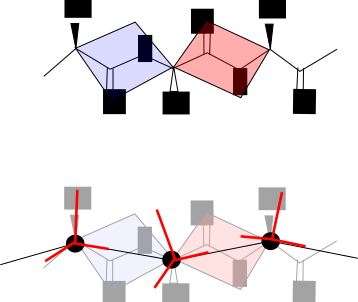
\includegraphics[width=\linewidth]{Fig/amide_planes.png}
    \caption{The model of protein using C-$\alpha$ atoms in internal coordinates.}
    \label{Fig:proteinModelCalpha}
\end{figure}

The position of the next atom in the chain is obtained by:
\begin{itemize}
\item Translation along axis x by 1\AA 
$$
T_x = \begin{bmatrix}
1 & 0 & 0 & 1 \\
0 & 1 & 0 & 0 \\
0 & 0 & 1 & 0 \\
0 & 0 & 0 & 1
\end{bmatrix} 
$$
\item Rotation by the angle $\alpha$ around the x axis (dihedral angle)
$$
R_x = \begin{bmatrix}
1 & 0 & 0 & 0 \\
0 & cos(\beta) & -sin(\beta) & 0 \\
0 & sin(\beta) & cos(\beta) & 0 \\
0 & 0 & 0 & 1
\end{bmatrix} 
$$
\item Rotation by the angle $\beta$ around the z axis (bending angle)
$$
R_z = \begin{bmatrix}
cos(\alpha) & -sin(\alpha) & 0 & 0 \\
sin(\alpha) & cos(\alpha) & 0 & 0 \\
0 & 0 & 1 & 0 \\
0 & 0 & 0 & 1
\end{bmatrix} 
$$

\end{itemize}

The first atom is fixed at the origin of coordinates. The total transformation matrix will look like:
$$
R = R_z \cdot R_x \cdot T_x = 
\begin{bmatrix}
cos(\alpha) & -sin(\alpha)cos(\beta) & sin(\alpha)sin(\beta) & cos(\alpha)\\
sin(\alpha) & cos(\alpha)cos(\beta) & -cos(\alpha)sin(\beta) & sin(\alpha)\\
0 & sin(\beta) & cos(\beta) & 0\\
0 & 0 & 0 & 1
\end{bmatrix} 
$$


Suppose we have $N_{angles}$ angles in the protein, they correspond to $N_{angles}+2$ vectors. The position of the first 
vector is fixed and the last vector is parametrized by the previous angle. To compute their positions we
sequentially multiply them by $R(\alpha_i, \beta_i) = R^i$:
$$ r_{i+1} = R^0 \cdot R^1 \dots A^{i-1} \cdot R^{i} \cdot \begin{bmatrix} 0 \\ 0 \\ 0 \\ 1 \end{bmatrix}$$
During the forward pass we save the matrixes:
$$A_i = R^{0} \cdot R^{1} \dots R^{i-1} \cdot R^{i}$$
because they are useful during backward computation. The coordinates of the atoms can be computed:
$$r_{i+1} = A_i \cdot \begin{bmatrix} 0 \\ 0 \\ 0 \\ 1 \end{bmatrix}$$

Now, we need to compute gradients of the internal angles with respect to the cartesian coordinates.
Each $R^{i}$ matrix depends on the angles $\alpha_i$ and $\beta_i$ (lets denote them as $q_i$), 
therefore the derivative of the coordinates:
$$ \frac{dr_i}{dq_j} = \frac{d R^{0} \cdot R^{1} \dots R^{i-1} \cdot R^{i} \cdot r_0} {dq_j} = 
R^{0} \cdot R^{1} \dots \frac{dR^j}{dq_j} \dots R^{i-1} \cdot R^{i} \cdot r_0 $$
using $A$ matrixes we obtain:
$$ \frac{dr_i}{dq_j} = A_{j-1}  \cdot \frac{dR^j}{dq_j} R^{j+1} \dots R^{i} \cdot r_0 $$




\subsection{From Euclidian space to Manifold}
\input{BMatrix.tex}

\bibliographystyle{plain}
\bibliography{VariationalMethods/citations,bibliography}

\end{document}
